 \section{Конструкторский раздел} \label{desing}

Важным этапом создания качественного и надежного приложения является проектирование базы данных. В данном разделе курсовой работы будет рассмотрено проектирование базы данных для разрабатываемого приложения. Будут выделены основные этапы проектирования, рассмотрены конкретные действия ролевой модели, спроектирован триггер и описаны основы проектирования приложения. Целью данного раздела является создание эффективной и масштабируемой базы данных, которая обеспечит стабильную работу приложения и удовлетворит потребности пользователей.

\subsection{Проектирование базы данных}

На основе выделенных ранее сущностей спроектированы следующие объекты базы данных.
\begin{enumerate}	
	\item Participant --- содержит информацию об участнике и имеет следующие поля:
	\begin{itemize}[label=---]
		\item participantId --- уникальный идентификатор участника;
		\item participantLastname --- фамилия участника;
		\item participantFirstname --- имя участника;
		\item participantPatronymic --- отчество участника;
		\item participantTeam --- команда участника;
		\item participantCity ---  город проживания участника;
		\item participantBirthday --- дата рождения участника;
		\item participantScore --- очки участника.
	\end{itemize}
	
	\item Team --- содержит информацию о команде и имеет следующие поля:
	\begin{itemize}[label=---]
		\item teamId --- уникальный идентификатор команды;
		\item teamName --- название команды;
		\item teamCompetitions --- соревнования, в которых принимает участие команда;
		\item teamScore --- очки команды.
	\end{itemize}
		
	\item Сompetition --- содержит информацию о соревновании и имеет следующие поля:
	\begin{itemize}[label=---]
		\item сompetitionId --- уникальный идентификатор соревнования;
		\item сompetitionName --- название соревнования;
		\item сompetitionTeams --- команды, участвующие в соревнованиях. 
	\end{itemize}	
	
	\item Step --- содержит информацию об этапе соревнования для участника:
	\begin{itemize}[label=---]
		\item stepId --- уникальный идентификатор этапа;
		\item stepName --- название этапа;
		\item stepParticipant --- участник, которому принадлежит этап; 
		\item stepCompetition --- соревнование, которому принадлежит этап; 
		\item lootScore --- очки за зачет.
	\end{itemize}
	
	\item Loot --- содержит информацию об улове участника:
	\begin{itemize}[label=---]
		\item lootId --- уникальный идентификатор улова;
		\item lootFish --- название рыбы;
		\item lootWeight --- вес рыб;
		\item lootStep --- зачет, к которому относится улов;
		\item lootScore --- очки за рыбу.
	\end{itemize}
	
	\item User --- содержит информацию о пользователе и имеет следующие поля:
	\begin{itemize}[label=---]
		\item userId --- уникальный идентификатор пользователя;
		\item userAuthorization --- авторизация пользователя;
		\item userRole ---  роль пользователя.
	\end{itemize}	
	
	\item Authorization --- содержит информацию об авторизации и имеет следующие поля:
	\begin{itemize}[label=---]
		\item authorizationId --- уникальный идентификатор авторизации;
		\item authorizationLogin --- логин;
		\item authorizationPassword ---  пароль.
	\end{itemize}	
\end{enumerate}

Соответствующая диаграмма по описанным выше данным представлена на рисунке \ref{fig:er} .

\begin{figure}[ht!]
	\centering{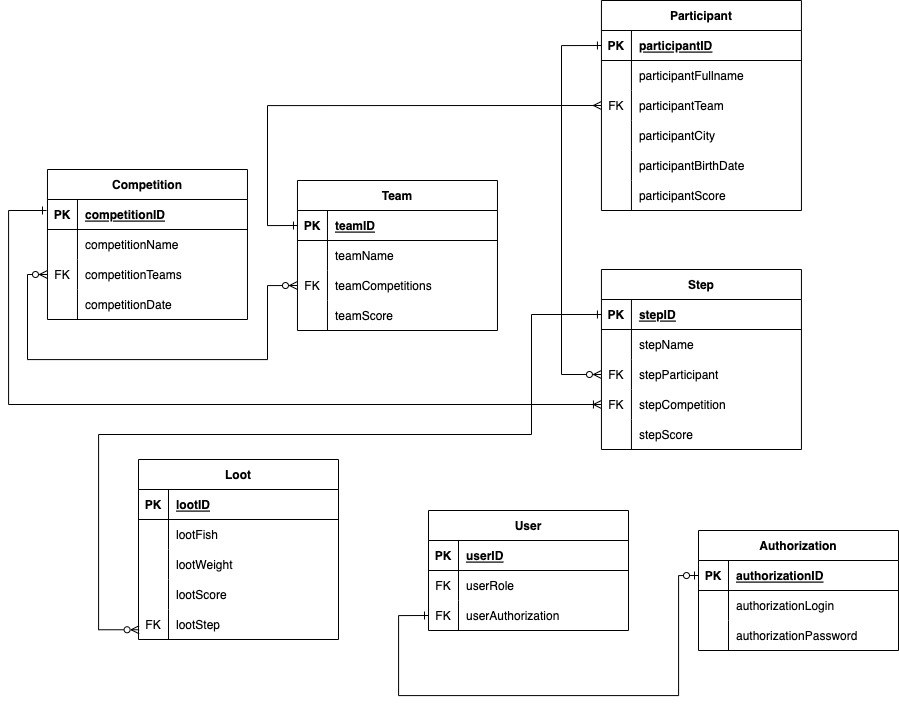
\includegraphics[scale=0.45]{img/er}}
	\caption{ER--диаграмма}
	\label{fig:er}
\end{figure}

\newpage


\subsection{Ролевая модель}

Ролевая модель предполагает наличие трех ролей: участника, судьи и администратора. Стоит отметить, что судья обладает всеми правами участника, а администратор --- всеми правами судьи.

Для успешной реализации поставленной задачи программа должна предоставлять следующие возможности:
\begin{itemize}[label=---]
	\item просмотр профилей участников;
	\item просмотр профилей команд;
	\item просмотр личного и командного рейтингов;
	\item просмотр личного и командного рейтингов по этапам;
	\item сортировка личного и командного рейтингов по убыванию/по возрастанию;
	\item сортировка личного и командного рейтингов по этапам по убыванию/по возрастанию.
\end{itemize}

Дополнительные возможности судьи:
\begin{itemize}[label=---]
	\item регистрация;
	\item авторизация;
	\item создание/удаление соревнования;
	\item создание/редактирование/удаление команды;
	\item создание/редактирование/удаление участника;
	\item создание/редактирование/удаление улова;
	\item добавление улова в этап;
	\item добавление участника в команду;
	\item добавление команды в соревнование.
\end{itemize}

Дополнительные возможности администратора:
\begin{itemize}[label=---]
	\item редактирование/удаление профилей судей;
	\item создание/редактирование/удаление профилей администраторов.
\end{itemize}

\subsection{Триггер}
Триггер --- это хранимая процедура особого типа, которую пользователь не вызывает непосредственно, а исполнение которой обусловлено действием по изменению данных: добавлением, модификацией, удалением строки в заданной таблице.  
 
В каждой из сущностей, таких как улов, этап, участник и команда, представлено поле «очки». Когда рыба взвешена и очки за нее необходимо добавить в этап участника, присвоить участнику и его команде, нужно в каждой сущности, связанной с уловом, обновить значение поля. 

Связи соответствующих сущностей представлены на рисунке \ref{fig:score}.

\begin{figure}[ht!]
	\centering{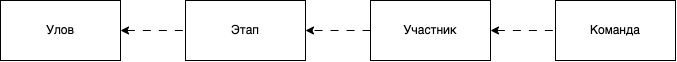
\includegraphics[scale=0.6]{img/score}}
	\caption{Диаграмма связей сущностей при обновлении очков}
	\label{fig:score}
\end{figure}

Для процедуры перерасчета очков было бы удобно создать триггер, который автоматически обновляет значение соответствующего поля в описанных четырех сущностях, при добавлении, редактировании и удалении улова.  

Схема алгоритма триггера представлена на рисунке \ref{fig:score}.

\begin{figure}[ht!]
	\centering{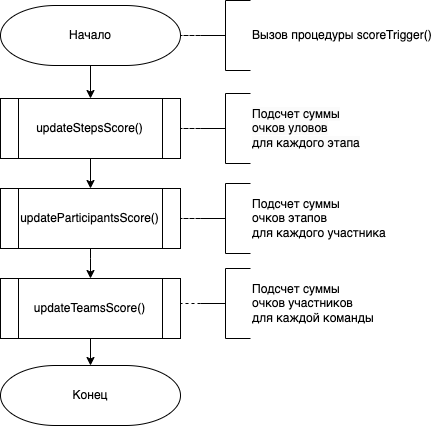
\includegraphics[scale=0.5]{img/trigger}}
	\caption{Триггер для обновления очков}
	\label{fig:trigger}
\end{figure}

\subsection{Проектирование приложения}

При разработке приложение для iOS может быть разделено на 3 этапа в соответствии с принципами «чистой архитектуры» \cite{cleanarc}:
\begin{enumerate}
	\item слой доступа к данным --- подключение к базе данных, отправка запросов, получение информации из базы данных;
	\item слой пользовательского интерфейса (UI) --- взаимодействие пользователя с программой;
	\item слой бизнес логики --- взаимодействия между слоем доступа к данным и приложением.
\end{enumerate}


\subsection{Вывод из раздела}

В результате проектирования базы данных для разрабатываемого приложения были выявлены и описаны основные этапы проектирования, которые позволили создать базу данных, удовлетворяющую требованиям. Были спроектированы сущности базы данных и их связи, ролевая модель и триггер, что обеспечило стабильную работу приложения и удовлетворило потребности пользователей. Были также формализованы требования к программе и описаны этапы разработки приложения, что позволит эффективно продолжить работу над проектом и достичь поставленных целей. 
